
\documentclass[a4paper]{article}

%Пакеты для математических символов:
\usepackage{amsmath} % американское математическое сообщество.
\usepackage{amssymb} % миллион разных значков и готический, ажурный шрифты.
\usepackage{amscd} % диаграммы, графики.
\usepackage{amsthm} % окружения теорем, определений и тд.
\usepackage{physics} % основные физические символы
%\usepackage{latexsym} % треугольники и пьяная стрелка.

%пакеты для шрифтов:
%\usepackage{euscript} % прописной шрифт с завитушками.
\usepackage{MnSymbol} % Значеки доказательства
\usepackage{verbatim} % улучшенный шрифт "пишущей машинки".
%\usepackage{array} % более удобные таблицы.
%\usepackage{multirow} % мультистолбцы в таблицах.
%\usepackage{longtable} % таблицы на несколько страниц.
%\usepackage{latexsym}

\usepackage{etoolbox}
\usepackage{slashbox} %Разделениени текста \backslashbox{}{}
\usepackage{collectbox} % Добавляет коробочки, можно складывать туда текст)


\usepackage{hyperref} % Ссылки как внешние так и внутренние
\hypersetup{
    colorlinks=true,
    linkcolor=black,
    filecolor=magenta,      
    urlcolor=cyan,
    pdftitle={Overleaf Example},
    pdfpagemode=FullScreen,
    }
    
%Пакеты для оформления:
\RequirePackage[center, medium]{titlesec}% Стиль секций и заголовков
%\usepackage[x11names]{xcolor} % 317 новых цветов для текста.
\usepackage{float} % Позволяет использовать H, h! для локации фигур
%\usepackage{multicol} % набор текста в несколько колонн.
\usepackage{graphicx} % расширенные возможности вставки стандартных картинок.
\usepackage{subcaption} % возможность вставлять картинки в строчку
%\usepackage{caption} % возможность подавить нумерацию у caption.
\usepackage{wrapfig} % вставка картинок и таблиц, обтекаемых текстом.
\usepackage{cancel} % значки для сокращения дробей, упрощения, стремления.
\usepackage{misccorr} % в заголовках появляется точка, но при ссылке на них ее нет.
%\usepackage{indentfirst} % отступ у первой строки раздела
%\usepackage{showkeys} % показывает label формул над их номером.
%\usepackage{fancyhdr} % удобное создание верхних и нижних колонтитулов.
%\usepackage{titlesec} % еще одно создание верхних и нижних колонтитулов

%Пакеты шрифтов, кодировок. НЕ МЕНЯТЬ РАСПОЛОЖЕНИЕ.
\usepackage[utf8]{inputenc} % кодировка символов.
%\usepackage{mathtext} % позволяет использовать русские буквы в формулах. НЕСОВМЕСТИМО С tempora.
\usepackage[T1, T2A]{fontenc} % кодировка шрифта.
\usepackage[english, russian]{babel} % доступные языки.

\usepackage{xcolor}
\definecolor{mycolor}{RGB}{244,228,215}

%Отступы и поля:
%размеры страницы А4 11.7x8.3in
\textwidth=7.3in % ширина текста
\textheight=10in % высота текста
\oddsidemargin=-0.5in % левый отступ(базовый 1дюйм + значение)
\topmargin=-0.5in % отступ сверху до колонтитула(базовый 1дюйм + значение)


%Сокращения
%Скобочки
\newcommand{\inrad}[1]{\left( #1 \right)}
\newcommand{\inner}[1]{\left( #1 \right)}
\newcommand{\infig}[1]{\left{ #1 \right}}
\newcommand{\insqr}[1]{\left[ #1 \right]}
\newcommand{\ave}[1]{\left\langle #1 \right\rangle}


%% Красивые <= и >=
\renewcommand{\geq}{\geqslant}
\renewcommand{\leq}{\leqslant}

%%Значек выполнятся
\newcommand{\per}{\hookrightarrow}

%%Векторная алгебра
\newcommand{\rot}{\text{rot}}
\renewcommand{\div}{\text{div}}
\renewcommand{\grad}{\text{grad}}

%% Более привычные греческие буквы
\renewcommand{\phi}{\varphi}
\renewcommand{\epsilon}{\varepsilon}
\newcommand{\eps}{\varepsilon}
\newcommand{\com}{\mathbb{C}}
\newcommand{\re}{\mathbb{R}}
\newcommand{\nat}{\mathbb{N}}
\newcommand{\stp}{$\filledmedtriangleleft$}
\newcommand{\enp}{$\filledmedsquare$}

\makeatletter
\newcommand{\sqbox}{%
    \collectbox{%
        \@tempdima=\dimexpr\width-\totalheight\relax
        \ifdim\@tempdima<\z@
            \fbox{\hbox{\hspace{-.5\@tempdima}\BOXCONTENT\hspace{-.5\@tempdima}}}%
        \else
            \ht\collectedbox=\dimexpr\ht\collectedbox+.5\@tempdima\relax
            \dp\collectedbox=\dimexpr\dp\collectedbox+.5\@tempdima\relax
            \fbox{\BOXCONTENT}%
        \fi
    }%
}
\makeatother
\newcommand{\mergelines}[2]{
\begin{tabular}{llp{.5\textwidth}}
#1 \\ #2
\end{tabular}
}
\newcommand\tab[1][0.51cm]{\hspace*{#1}}
\newcommand\difh[2]{\frac{\partial #1}{\partial #2}}
\newcommand{\messageforpeople}[1]{HSE Faculty of Physics \ \ HSE Faculty of Physics HSE Faculty of Physics \ \ HSE Faculty of Physics HSE Faculty of Physics \ \ HSE Faculty of Physics HSE Faculty of Physics \ \ HSE Faculty of Physics HSE Faculty of Physics \ \ HSE Faculty of Physics HSE Faculty of Physics \ \ HSE Faculty of Physics HSE Faculty of Physics \ \ HSE Faculty of Physics HSE Faculty of Physics \ \ HSE Faculty of Physics }


\numberwithin{equation}{section}

\begin{document}

\begin{flushright}
    Выполнил:
    Карибджанов Матвей

    Вариант:
    22
\end{flushright}
\tableofcontents
\newpagestyle{main}{
\setfootrule{0.4pt}
\setfoot{}{\thepage}{\sectiontitle}}
\pagestyle{main}


\section{Задание}

Решаю задачу в "CW\_2.ipynb", так что здесь будут перевелены только формулы и ответы. В программе я матрици не округляю в памяти они храняться 
с той точносью с которой были посчитаны, поэтому в решения ответы с использованием округленных матриц могут оличаться от тех, что были посчитаны
в программе.

Нахожу обратную к матрице $A$:
\begin{gather}
    A^{-1} = 
    \begin{pmatrix}
        -3& 2\\
        6& -8
    \end{pmatrix} ^{-1}
    = 
    \begin{pmatrix}
        -0.67 & 0.17\\ 
        0.5 & -0.25
    \end{pmatrix}    
\end{gather}

Оценим погрешность найденного решения сверху:


\begin{gather}
    \delta A^{-1} \leq \cfrac{\norm{Y}}{1 - \norm{Y}} = 0.02; \ \norm{Y} \leq \norm{\delta A}\norm{A^{-1}} 
\end{gather}





\section{Задание}

Мне показалось логично округлять до целых, так как матрица остается не вырожденной
но при этом становится диагональной, из-за чего легко искать обратную. 
\begin{gather}
    A = 
    \begin{pmatrix}
        -5.0 & 0\\ 
        0 & -1.0
    \end{pmatrix}
    ;
    \
    \Delta A =
    \begin{pmatrix}
        0.03 & -0.14\\ 
        -0.06 & 0.04
    \end{pmatrix}
\end{gather}
\begin{gather}
    b = 
    \begin{pmatrix}
        -5.0\\ 
        -1.0
    \end{pmatrix};
    \
    \Delta b = 
    \begin{pmatrix}
        -0.18\\ 
        -0.08
    \end{pmatrix}
\end{gather}
\begin{gather}
    A^{-1} =
    \begin{pmatrix}
        -0.2 & 0\\ 
        0 & -1.0
    \end{pmatrix}
\end{gather}

Таким образом число обусловленности и погрешность $d$:
\begin{eqnarray}
    \kappa_1 \inner{A} = 5, & \kappa_2 \inner{A} = 5 \\
    \delta_1 b = 23.08, & \delta_2 b = 25.89
\end{eqnarray}

Я получил погрешность:
\begin{eqnarray}
    5.18 \leq &\delta_1 x& \leq 115.38 \\
    5.18 \leq &\delta_2 x& \leq 129.43
\end{eqnarray}

Предлагаю посчитаь точно и убедиться в этом, 
не буду пояснять поск решений просто приведу результат:
\begin{gather}
    x_{real} = \begin{pmatrix}
        1.08\\ 
        1.19
    \end{pmatrix},
    \
    x = 
    \begin{pmatrix}
        1.0\\ 
        1.0
    \end{pmatrix},
    \
    \Delta x = 
    \begin{pmatrix}
        0.08\\ 
        0.19
    \end{pmatrix}
\end{gather}

Тогда получим натоящюю погрешность:
\begin{equation}
    \delta_1 x = 7.46, \
    \delta_2 x = 6.84
\end{equation}

Действительно $\delta_1 x$ и $\delta_2 x$ лежет в найденных интервалах.



\section{Задание}

По алгоритму PageRank получил самую влиятельную вершину графа - 4.


\begin{figure}[H]
    \centering
    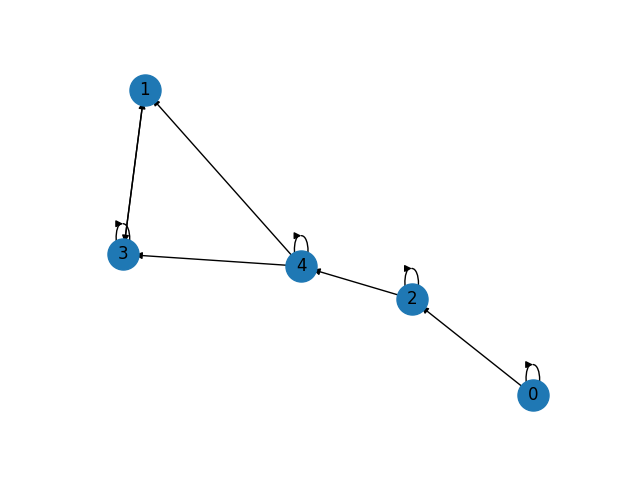
\includegraphics[trim={0 0 0 0},clip,width=\textwidth]{Imgs/graph.png}
    \label{graph}
\end{figure}










\end{document}